\documentclass{article}

%
% 引入模板的style文件
%
\usepackage{homework}
\usepackage{enumitem}  % 允许对列表间距修改
\usepackage[colorlinks,linkcolor=red]{hyperref}  % 允许插入超链接
%
% 封面
%

\title{
	
\includegraphics[scale = 0.45]{images/title/ucas-logo.png}\\
    \vspace{1in}
    \textmd{\textbf{\hmwkClass\ \hmwkTitle}}\\
    \textmd{\textbf{\hmwkSubTitle}}\\
    \normalsize\vspace{0.1in}\small{\hmwkCompleteTime }\\
    \vspace{0.1in}\large{\textit{\hmwkClassInstructor\ }}\\
    \vspace{3in}
}

\author{\hmwkAuthorName}
\date{}

\renewcommand{\part}[1]{\textbf{\large Part \Alph{partCounter}}\stepcounter{partCounter}\\}


%
% 正文部分
%
\begin{document}


\maketitle

\pagebreak

\section{1. 一级标题}
\subsection{1.1 二级标题}
\subsubsection{1.1.1 三级标题}
\section{2. 项目列表} 
\subsection{2.1 无序列表}

默认带有原点
\begin{itemize}
	\item hello, how are you?
	\item 你好,我是cp
\end{itemize} 
修改原点为其他 
\begin{itemize}
	\item[-] hello, how are you?
	\item[*] 你好,我是cp
	\item[] 消除原点
\end{itemize} 


\subsection{2.2 有序列表} 

\begin{enumerate}
	\item 默认1
	\item 默认2
	\item 默认3
\end{enumerate}

利用无序手动更改为有序,并进行缩进
\begin{itemize}[itemindent=1em]
	\item[(1)] 手动有序1
	\item[(2)] 手动有序2
	\item[(3)] 手动有序3
\end{itemize} 
与上间距
\begin{itemize}[itemindent= 15 pt]
	\item[step 1] 手动有序1
	\item[step 2] 手动有序2
	\item[step 3] 手动有序3
\end{itemize} 
更多间距调整内容参考\href{https://blog.csdn.net/robert_chen1988/article/details/83179571}{latex 列表间距修改} 

\section{3. 公式}
\subsection{3.1 无编号公式}

多行公式
\[
\begin{split}
n^2 + n + 1 &=
\\
&\leq n^2 + n^2 + n^2
\\
&= 3n^2
\\
&\leq c \cdot 2n^3
\end{split}
\]
行内公式

后面是个公式\(f(n) = n^2 + n + 1\), \(g(n) = 2n^3\)

\subsection{3.2 带编号公式}
\begin{equation}
\begin{split}
z_o = \sigma(W_o*(x_t,h_{t-1}))\\
z_f = \sigma(W_f*(x_t,h_{t-1}))\\
z_i = \sigma(W_i*(x_t,h_{t-1}))\\
z = \tanh(W*(x_t,h_{t-1}))
\end{split}
\end{equation}

\section{4. 代码}
\begin{lstlisting}[language = python, numbers=left, 
numberstyle=\tiny,keywordstyle=\color{blue!70},
commentstyle=\color{red!50!green!50!blue!50},frame=shadowbox,
rulesepcolor=\color{red!20!green!20!blue!20},basicstyle=\ttfamily]

# 这是注释
def test():
  pass

\end{lstlisting}

\section{5. 图片} 
\begin{figure}[H]
	\centering
	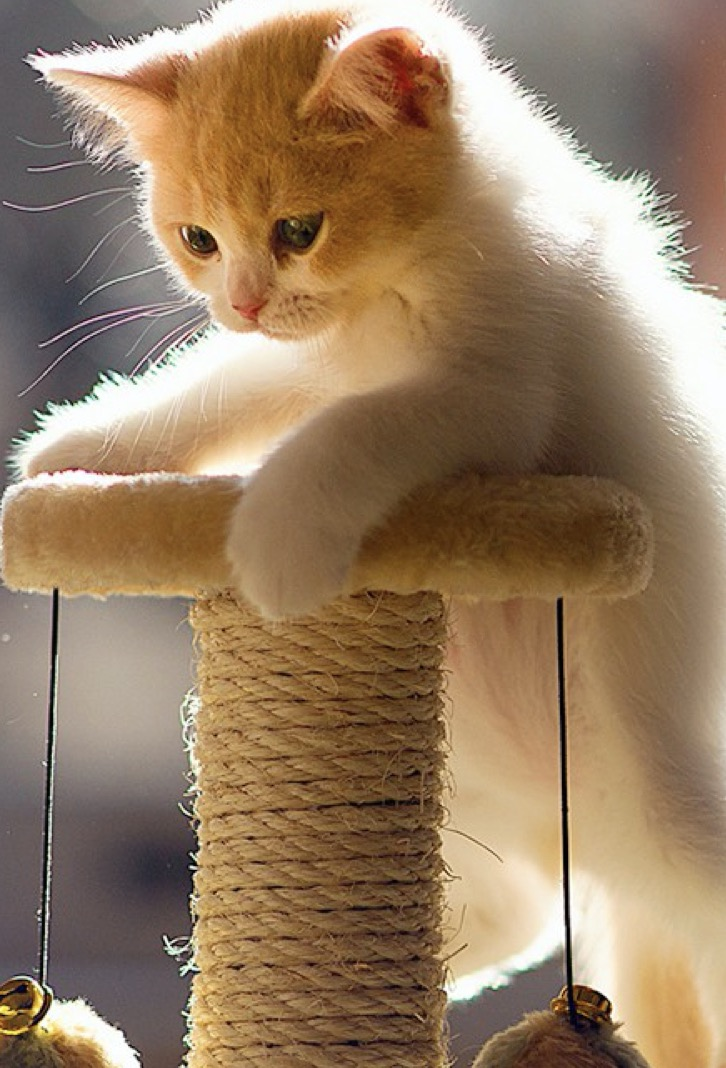
\includegraphics[width=0.3\linewidth]{images/test-fig.png}
	\caption{LSTM基本结构单元}
	\label{fig:LSTM基本结构单元}
\end{figure}

\section{6. 表格} 
算法
\begin{algorithm}[H]
	\begin{algorithmic}[1] %每行显示行号
		\Require{Positive Instance Set $ P $, Unlabeled Instance Set $ U $ , Sample Ratio s.}
		\Ensure{Reliable Negative Instance Set $ RN $.}
		
		\State{$set  RN = \emptyset $}
		\State{Sample $ s $ of the instances from $ P $ as $ S $}
		\State{Set $ P_s  = P − S$ with label $ 1 $, $ U_s = U \cup S $ with label $ -1 $}
		\State{Train a classifier $ g $ with $ P_s $ and $ U_s $}
		\State{Classify instances in $ U $ using $ g $, output the class-conditional-probability}
		\State{Select a threshold $ \theta $ according to the class-conditional-probability of
			instances in $ S $}
		\For{$ d \in U $ do}
		\If{$ Pr(1|d) \leq \theta, RN = RN \cup d $}
		\EndIf
		\EndFor
		\State{Output RN}
	\end{algorithmic}
	\caption{Reliable Negative Instances Selection}
	\label{alg:Reliable Negative Instances Selection}
\end{algorithm}

表格1 

\begin{tabular}{|c|c|c|c|}
	\hline 
	方法 & 特点 & 优点 & 缺点  \\ 
	\hline 
	有监督学习 & \tabincell{c}{对数据进行标注,\\ 通过有监督学习的方式\\ 来检测恶意URL} & 更强的泛化能力 & \tabincell{l}{现实生活中很难获得\\ 精准的标注数据。\\ 在更多时候,我们可能\\ 只得到一小部分恶意URL\\ 和大量未标记的URL样本,\\ 缺乏足够可靠的负例样本} \\ 
	\hline 
	无监督学习 & 不需要对数据进行标注 & 无需标注的数据即可进行训练 & \tabincell{c}{已知恶意URL的标注信息\\ 就难以充分利用,可能\\ 无法达到令人满意的识别能力} \\
	\hline
\end{tabular}  

表格2

\begin{tabular}{ccc}
	\hline
	姓名& 学号& 性别\\
	\hline
	Steve Jobs& 001& Male\\
	Bill Gates& 002& Female\\
	\hline
\end{tabular}

表格3带编号
\begin{table}[ht]
	\caption{表格哈哈哈哈}
	\centering
	\begin{tabular}{c || c | c | c | c | c}
		& \(x \mod 5 = 0\)
		& \(x \mod 5 = 1\)
		& \(x \mod 5 = 2\)
		& \(x \mod 5 = 3\)
		& \(x \mod 5 = 4\)
		\\
		\hline
		\(x0\) & 0 & 2 & 4 & 1 & 3 \\
		\(x1\) & 1 & 3 & 0 & 2 & 4 \\
	\end{tabular}
\end{table}


更多表格样式参考:\href{https://www.jianshu.com/p/35abc6772576}{表格样式} 


\section{7. 参考文献}
参考文献:\cite{cup2007available} 

% 引用文献
\bibliographystyle{unsrt}  % unsrt:根据引用顺序编号
\bibliography{refs}

\end{document}
